\documentclass[luatex,mathserif,serif]{beamer}

\usepackage{polyglossia}

% Установка язков
\setdefaultlanguage{russian}
\setmainlanguage{russian}
\setotherlanguage{english}

% Лигатуры нужны для правильного отображения тире, кавычек и прочего
\setmainfont[Ligatures=TeX]{Times New Roman}
\setmonofont[Ligatures=TeX]{Courier New}

% Необходимо для киррилических шрифтов
\newfontfamily{\cyrillicfont}[Ligatures=TeX]{Times New Roman}
\newfontfamily{\cyrillicfonttt}[Ligatures=TeX]{Courier New}

\usepackage{graphicx}
\DeclareGraphicsExtensions{.pdf,.png,.jpg,.eps}
\graphicspath{{figures/}}

% Зачем: Учет особенностей различных языков.
\usepackage{babel}


\usetheme{Warsaw}


\begin{document}
\title[Система ФКУ КМУ артиллерийского дивизиона] % (optional, only for long titles)
{Система функционального контроля технических средств комплекса машин управления артиллерийского дивизиона}
\author % (optional, for multiple authors)
{Стаховский А. В.}
\institute
{
	\inst{}
  БГУИР
}

\frame{\titlepage}

\begin{frame}
	\frametitle{Цель дипломного проекта}
	Разработка и реализация системы автоматизации процессов тестирования
	технических средств и каналов обмена данными в локальной сети, а также  упрощение ведения отчетности.
\end{frame}

\begin{frame}
	\frametitle{Задачи}
	Для успешного выполнения поставленной цели, работа над проектом была разбита на следующие задачи:
	\begin{itemize}
		\item выбор технологий, удовлетворяющих требованиям;
		\item разработка управляющего модуля;
		\item разработка алгоритмов функционального контроля:
			\begin{itemize}
				\item навигационной системы,
				\item метеостанции,
				\item радиостанции,
				\item прибора наблюдения разведчика <<Капонир>>,
				\item лазерного целеуказателя-дальномера,
				\item принтера;
			\end{itemize}
		\item разработка алгоритмов журналирования;
		\item разработка программы для просмотра журнала тестирования.
	\end{itemize}
\end{frame}

\begin{frame}
	\frametitle{Машина начальника штаба дивизиона на колесном шасси}
	\begin{figure}
		\centering
		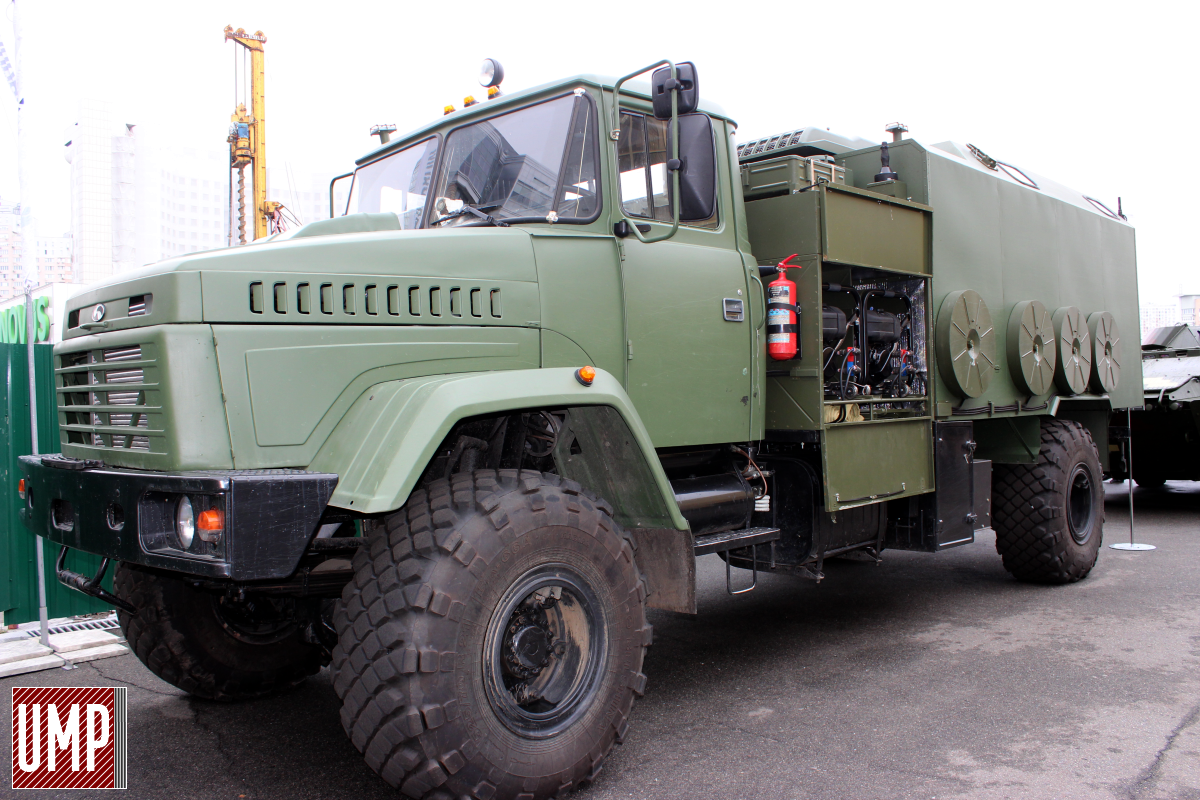
\includegraphics[scale=0.25]{div_com}
	\end{figure}
\end{frame}

\begin{frame}
	\frametitle{Автоматизированное рабочее место}
	\begin{figure}[ht]
		\centering
		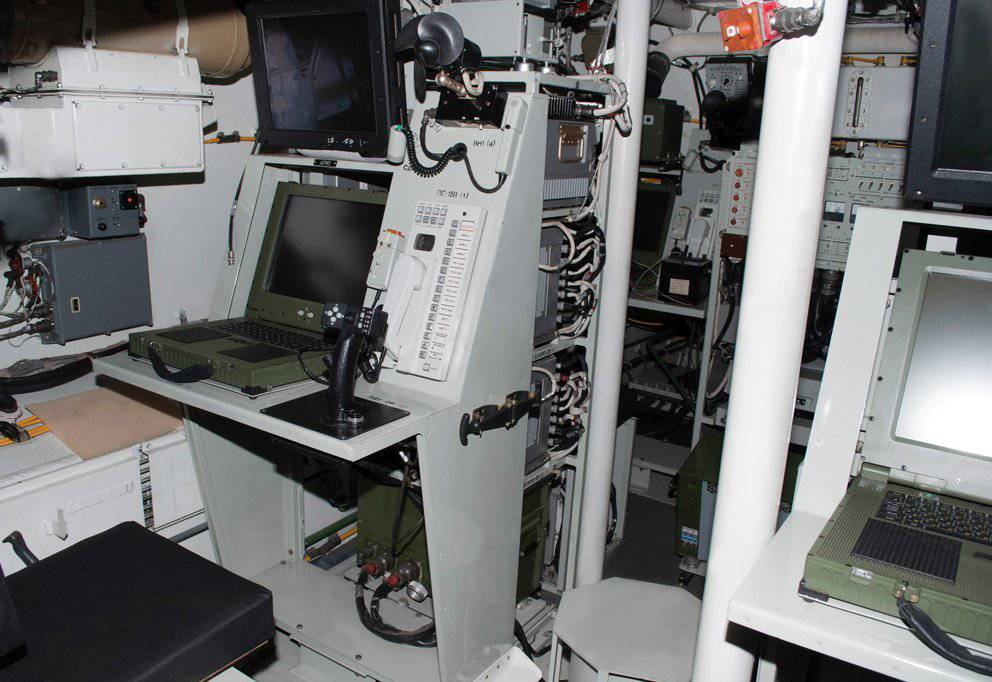
\includegraphics[scale=0.30]{arm}
	\end{figure}
\end{frame}

\begin{frame}
	\frametitle{База дипломного проекта}
	\begin{figure}[ht]
		\centering
		
\includegraphics[scale=0.5]{agat}
	\end{figure}
\end{frame}
\end{document}
